%==============================================================================
\documentclass[]{buthesis}
%==============================================================================


%==============================================================================
% ----------------- DOCUMENT INFORMATION FOR PDF CREATION ---------------------
\def\Author{Sir Isaac Netwon}
\def\Title{Differential Equations of the form $^2$H$_{2-x}$O$_x$}
% ----------------------------
\def\Year{2022}
\def\Month{01}
\def\Day{31}
% ----------------------------
\def\Subtitle{}
\def\Subject{}
\def\Keywords{Brock University, Physics} % COMMA SEPARATED LIST OF KEY WORDS/PHRASES
% ----------------------------
\def\URL{https://www.overleaf.com/read/rhzhgfkfhypy} % SHARE URL TO OVERLEAF PROJECT
% ----------------------------
\toggletrue{use-cc-license}
%\togglefalse{use-cc-license}
\makepdfa
%==============================================================================


%==============================================================================
\addbibresource{my_bibliography.bib} % Imports bibliography file
%==============================================================================


%==============================================================================
\begin{document}
%==============================================================================


%==============================================================================
% Monograph Format
% Prefatory pages:
%==============================================================================
% Frontispiece or Quote Page (optional)
%
\clearpage
\thispagestyle{empty}
\begin{quote}
``To any action there is always an opposite and equal reaction; in other words, the actions of two bodies upon each other are always equal and always opposite in direction.''\\
---  \emph{The Principia: Mathematical Principles of Natural Philosophy} (1687)
\end{quote}
%==============================================================================


%==============================================================================
% Title Page
%
\clearpage
\maketitle
%==============================================================================


%==============================================================================
% Dedication (optional)
%
\clearpage
\section*{Dedication}
In a dedication, the student honors the persons involved in the process of writing the thesis paper. It's an act of gratitude to all those persons in your life who have a role in the writing journey.

Dedicated to Isaac Barrow, (b. October 1630, London, England --- d. May 4, 1677, London), English classical scholar, theologian, and mathematician.
%==============================================================================


%==============================================================================
% Abstract
%
\clearpage
{\setstretch{2.0}
\section*{Abstract}

The thesis abstract is an essential part of the dissertation paper. It is a summary of a complete work. It gives readers a chance to discover the key points of your dissertation, its research chapter, methodology and results part. Writing a proper abstract is important.

\kant[11]
}
%==============================================================================


%==============================================================================
% Preface (optional) 
%
\clearpage
\section*{Preface}
A preface is an introductory passage written about a book by its author. It lays out why the book exists, its subject matter, and its goals. Prefaces are more commonly found in nonfiction books, but they can also be used in fiction.
%==============================================================================


%==============================================================================
% Acknowledgement (optional) 
%
\clearpage
\section*{Acknowledgement}
The acknowledgement for thesis is the section where you thank all people, institutions, and companies that helped you complete the project successfully. It is similar to a dedication, except for the fact that it is formal.
%==============================================================================


%==============================================================================
% Table of contents
%
\clearpage
\tableofcontents
%==============================================================================


%==============================================================================
% List of figures (if any)
%
\clearpage
\listoffigures
%==============================================================================


%==============================================================================
% List of tables (if any)
%
\clearpage
\listoftables
%==============================================================================


%==============================================================================
% List of Symbols, Nomenclature, or Abbreviations (if any)  
%
\clearpage
\section*{List of Symbols and Abbreviations}
\begin{description}
\item[$\omega$]{Angular acceleration}
\item[$\Phi$]{Quantum mechanical wave function.  A wave function in quantum physics is a mathematical description of the quantum state of an isolated quantum system. The wave function is a complex-valued probability amplitude, and the probabilities for the possible results of measurements made on the system can be derived from it.}
\item[\emph{Impulse}]{In classical mechanics, impulse (symbolized by $J$ or Imp) is the integral of a force, $F$, over the time interval, $t$, for which it acts.}
\item[NSERC]{National Science and Engineering Research Council}
\end{description}
%==============================================================================


%==============================================================================
%
% Main text
%
\clearpage
\pagenumbering{arabic}
\setcounter{page}{1}
\fancyhead[R]{\thepage}
\fancyhead[L]{\nouppercase{\S\leftmark}}
%==============================================================================
% 
\section{Introduction}\label{section:introduction}

\kant[1] 

In this paragraph, we show how you can reference an equation, such as Gauss's Law in integral form shown in Equation~\ref{eq:gauss_law_integral_form}. 

% =======================================================
\begin{equation}
\label{eq:gauss_law_integral_form}
\mathbf{E} \cdot \mathrm{d}\mathbf{S} ={\frac{1}{\varepsilon_{0}}}\iiint_{\Omega}\rho\,\mathrm{d}V
\end{equation}
% =======================================================

\kant[2] 

In this paragraph, I am including some numerical results with and without units, inline with the text. Some examples would be; \complexnum{1+-2i} for complex numbers,
\num{.3e45}~\unit{\kilogram\metre\per\second} for a scientific notation, and 
\qtylist{0.13;0.67;0.80}{\milli\metre} for a list of answers. Below we show an answer in a math equation environment.

% =======================================================
\begin{equation}
\label{eq:numbers_and_units}
\mathbf{E} = \num{1.2e-12}\ \unit{kg.m.s^{-1}}
\end{equation}
% =======================================================


The Maxwell/Faraday equation in integral form is shown in equation~\ref{eq:maxwell_faraday_equation_integral_form}

% =======================================================
\begin{equation}
\label{eq:maxwell_faraday_equation_integral_form}
\oint_{\partial\Sigma} \mathbf{E} \cdot \mathrm{d}{\mathbf{\ell}}=-{\frac {\mathrm{d}}{\mathrm{d}t}} \iint_{\Sigma}\mathbf{B}\cdot\mathrm{d}\mathbf{S} 
\end{equation}
% =======================================================

Using \texttt{biblatex} you can display bibliography divided into sections,  depending of citation type. Let's cite! The Einstein's journal paper \cite{einstein} and the Dirac's book \cite{dirac} are physics related items. Next, \textit{The \textsc{latex} Companion} book \cite{latexcompanion}, the Donald Knuth's website \cite{knuthwebsite}, \textit{The Comprehensive Tex Archive Network} (CTAN) \cite{ctan} are \textsc{latex} related items; but the others Donald Knuth's items \cite{knuth-fa,knuth-acp} are dedicated to programming. 



%==============================================================================
% 
\section{Methods}\label{section:methods}
\kant[5]

\subsection{Technique 1}
\kant[6]

% =======================================================
\begin{equation}\label{eq:entropy}
S=-k_{\textrm{B}}\sum_{i}\rho_{i}\ln\rho_{i}
\end{equation}
% =======================================================

\kant[7]

% =======================================================
\begin{figure}[h]\label{fig:test_inset}
\begin{center}
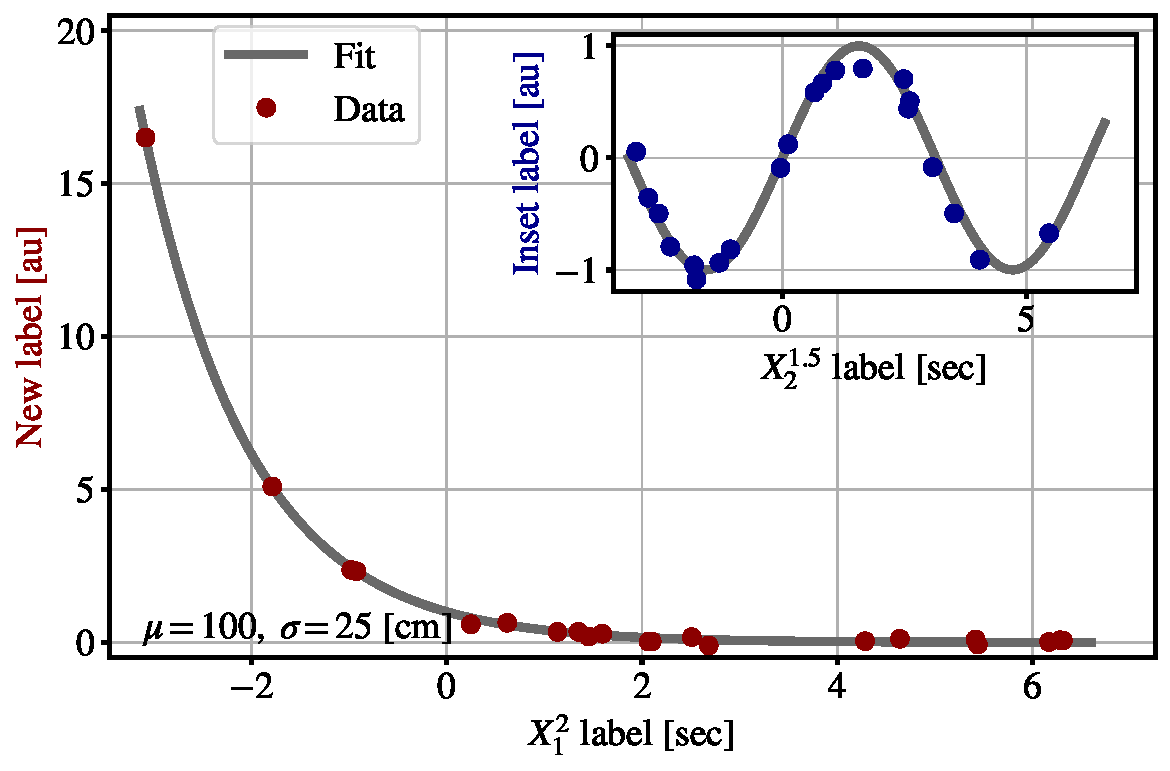
\includegraphics[scale=0.6]{figures/test_inset.pdf}
\end{center}
\caption{This is a test figure with an inset.}
\end{figure}
% =======================================================

\kant[8] And there's more to be written about this topic.~\cite{einstein}

% =======================================================
\begin{table}[h]\label{tab:zoo_animal_prices}
\begin{center}\begin{tabular}{llr}
\toprule
\multicolumn{2}{c}{Item} \\
\cmidrule(r){1-2}
Animal    & Description & Price (\$) \\
\midrule
Gnat      & per gram    & 13.65      \\
          &    each     & 0.01       \\
Gnu       & stuffed     & 92.50      \\
Emu       & stuffed     & 33.33      \\
Armadillo & frozen      & 8.99       \\
\bottomrule
\end{tabular}\end{center}
\caption{Example of current zoo animal prices.}
\end{table}
% =======================================================

\kant[9]

%==============================================================================
%
\printbibliography[heading=bibnumbered]
\printbibliography[heading=subbibnumbered,
                   keyword={physics},
                   title={Physics-related only}]
%==============================================================================



%==============================================================================
\end{document}
